% ! Mode:: "TeX:UTF-8"
% ! Tex program = xelatex

\documentclass[aspectratio=169]{beamer}
\usepackage[utf8]{inputenc}
\usepackage[T1]{fontenc}
\usepackage{listings}%列表用到
 \lstset{%
  basicstyle=\small\ttfamily,
  language=[LaTeX]{TeX},
  %commentstyle=\color{hghred},keywordstyle=\color{hghblue},breaklines=true
 }
\usepackage{setspace}%调整行距用到
\usepackage{booktabs}%三线表用到
\usepackage{amsmath}%可以使用 align 环境
%\usepackage{ragged2e}%两端对齐用
\renewcommand{\raggedright}{\leftskip=0pt \rightskip=0pt plus 0cm}%需要的时候用 \raggedright 即可
\usepackage{subfigure}




\usetheme{hgh}

%\usepackage{pgfpages}
%\setbeameroption{show notes on second screen}


%改变默认字体
\usefonttheme{professionalfonts} % 使用 non standard fonts
%\usefonttheme{serif} % default family is serif
%\setmainfont{Times New Roman}%Times New Roman

%%%%%%%%%%% 设置中文 %%%%%%%%%%%%%
\usepackage{xeCJK}
\setCJKmainfont[AutoFakeSlant=0.3, AutoFakeBold=3]{FZShuSong-Z01S}%大部分中文不支持斜体、粗体,通过此命令实现

%以下两种方法可以实现公示字体类似 Times New Roman
%\usepackage{times}
%\usepackage{mathptmx}

\usepackage{newtxtext,newtxmath}
\usepackage{bm}


\usepackage{microtype}% microtype 宏包可以改善了单词、字母的间距,如果有使用到字体宏包,需要将 microtype 宏包放在它们的后面,因为这个宏包对单词、字母的调整和字体是有关的。
\usepackage{siunitx}% SI{10}{\hertz} 输出为 “10Hz”;\SIrange{10}{100}{\hertz} 输出为 “10Hz to 100Hz”。

\setbeamersize{text margin left=0.65cm, text margin right=0.65cm}%设置页边距
%%%%%%%%%%%%%%%%%%%%%%%%%%%%%%%%%

\title[非线性 Schr\"odinger 方程的数值模拟]{非线性 Schr\"odinger 方程的数值模拟}
\subtitle[作者]{作者}
\author{答辩人:韩旭东\\指导老师:王恒}
\institute{专业:应用物理学}
\date{\zhtoday}

%可以选择显示 section number 或者不显示
%\AtBeginSection{\frame{\sectionpage}}
\AtBeginSection{
  \let\insertsectionnumber\relax
%  \let\sectionname\relax
  \frame{\sectionpage}
}


%\setbeamercovered{dynamic}  % \pause 之后半透明
\begin{document}
\begin{frame}[noframenumbering,plain]
\titlepage
\end{frame}

\begin{frame}
  \frametitle{大纲}

  \centering

  \begin{minipage}{.75\textwidth}
 
    \setstretch{1.5}
  
        \tableofcontents
%如果节比较多,可以分两栏
%    \begin{columns}[t]
%      \begin{column}{.5\textwidth}
%        \tableofcontents[sections={1-5}]
%      \end{column}
%      \begin{column}{.5\textwidth}
%        \tableofcontents[sections={6-10}]
%      \end{column}
%    \end{columns}

  \end{minipage}  
\end{frame}

\section{研究背景}
\begin{frame}{非线性 Schr\"odinger 方程}
  \begin{block}{非线性 Schr\"odinger 方程\upcite{Agrawal}}
    描述短脉冲在光纤中传播时,包络随传输变化的方程。光纤主要材质是一种色散介质,短脉冲会在很小的时空尺度内会聚很高的能量。在色散效应和非线性效应的相互作用下,脉冲在光纤中的传输方程
    $$
      i\frac{\partial A}{\partial z}=\frac{\beta_2}{2}\frac{\partial^2A}{\partial T^2}-\gamma|A|^2A
    $$
  \end{block}
  \begin{block}{光学孤子效应\upcite{Hasegawa}}
    Hasegawa 和 Tappert 在 1973 年指出,反常群速度色散和非线性效应的相互作用使得孤子脉冲可以在低损光纤中传输,并通过数值实验证实了光孤子在通信系统中的稳定性。光孤子通信的广阔前景引起人们的兴趣,对它进行了广泛的研究。
  \end{block}  
\end{frame}




\begin{frame}{光孤子的物理图像}
  对于基阶孤子,自相位调制和色散影响互相平衡,脉冲的形状和频谱几乎不随传输变化。对于二阶、三阶甚至更高阶的孤子,自相位调制和群速度色散的影响地位是交替变化着的,导致传输过程中出现\textcolor{hghgreen}{脉冲变窄、分裂、再恢复的周期性演化结果}\upcite{Agrawal}。
  \begin{figure}[tbp]
    \centering
    \addtocounter{figure}{-1}
    \subfigure{
      \begin{minipage}[t]{0.3\linewidth}
        \includegraphics[width=1\linewidth]{基阶孤子无畸变传输.png}
        \caption{基阶孤子}
      \end{minipage}
    }
    \subfigure{
      \begin{minipage}[t]{0.3\linewidth}
        \includegraphics[width=1\linewidth]{二阶孤子解析解.png}
        \caption{二阶孤子}
      \end{minipage}
    }
    \subfigure{
      \begin{minipage}[t]{0.3\linewidth}
        \includegraphics[width=1\linewidth]{三阶孤子演化_时域.png}
        \caption{三阶孤子}
      \end{minipage}
    }
  \end{figure}
\end{frame}

\begin{frame}{本文工作}
  \begin{block}{数值求解的必要性}
    可用逆散射方法求解非线性 Schr\"odinger 方程得到脉冲传输的解析解(其中一种特殊情况就是光孤子解),但是需要求解复杂的积分方程。所以用解析方法只能得到特殊情形的结果,数值方法求解非线性 Schr\"odinger 方程是有必要的。
  \end{block}
  \begin{exampleblock}{非线性 Schr\"odinger 方程的数值求解}
    \begin{itemize}
      \item 通过频谱间接求解,\textcolor{hghred}{分步 Fourier 方法}和\textcolor{hghred}{伪谱方法};
      \item 在时域中直接求解,\textcolor{hghred}{有限差分法}。
    \end{itemize}
  \end{exampleblock}
  \begin{alertblock}{本文主要工作}
    本文\textcolor{hghpurple}{用 MATLAB }实现了\textcolor{hghred}{三种方法}数值求解非线性 Schr\"odinger 方程,\textcolor{hghgreen}{得到了单光孤子传输过程中周期性演化的物理图像}。
  \end{alertblock}
\end{frame}

\section{数值方法}
\begin{frame}{伪谱方法}
    \only<1>{
      \begin{columns}
      \column{.5\textwidth}
      Fourier 积分变换可以把时域(或空间域)的偏微分方程转换为频域的常微分方程,
      通过求解频域的常微分方程,再进行逆 Fourier 变换得到偏微分方程的时域(空间域)的解(见图\ref{fig:Fourier})。将此方法应用于偏微分方程离散求解,就是伪谱方法\upcite{zhangxiao,liangkunmiao}。
      \column{.4\textwidth}
      \begin{figure}
        \centering
        \setcounter{figure}{3}
        \includegraphics[width=1\linewidth]{线性傅里叶变换.png}
        \caption{Fourier 变换法解偏微分方程}
        \label{fig:Fourier}
      \end{figure}
    \end{columns}
    }
    \only<2>{
      通常非线性 Schr\"odinger 做时域 Fourier 变换
      \begin{align}
        &\frac{\partial \widetilde{u}}{\partial \xi}=-\frac{i\omega^2}{2}\widetilde{u}+i\mathscr{F}\left[\left|\mathscr{F}^{-1}[\widetilde{u}]\right|^2\mathscr{F}^{-1}[\widetilde{u}]\right] \nonumber \\
        &\widetilde{u}(0,\omega)=\mathscr{F}\left[N\cdot\mathrm{sech}(\tau)\right] \nonumber
      \end{align}
      通过数值求解频域的常微分方程,再经 Fourier 逆变换得到光孤子脉冲时域的传输结果。
      \begin{exampleblock}{两个数值问题\upcite{zhangxiao}}
        \begin{itemize}
          \item 离散 Fourier 变换 $\Rightarrow$ FFT 算法 $\Rightarrow$ fft 与 ifft 函数
          \item 常微分方程的数值求解 $\Rightarrow$ Runge-Kutta 方法 $\Rightarrow$ ode45 求解器
        \end{itemize}
      \end{exampleblock}
    }
\end{frame}

\begin{frame}{分步 Fourier 方法}
  \only<1>{
    分步 Fourier 方法假设光场传输过程中色散作用和非线性作用交替进行,分别考虑其影响,从而得到光波传输的近似结果。脉冲从 $z$ 到 $z+h$ 传播一小段距离,可做近似
    $$
      A(z+h,T)\approx\exp(h\hat{D})\exp(h\hat{N})A(z,T)
    $$
    非线性效应的影响可以在时域中计算,色散效应的影响在频域中计算更为方便
    $$
      \exp(h\hat{D})B(z,T)=\mathscr{F}^{-1}\left[\exp(h\hat{D}(-i\omega))\mathscr{F}[B(z,T)]\right]
    $$
    其中,$\hat{D}(-i\omega)$ 表示用 $-i\omega$ 去替换时域微分算子 $\partial/\partial T$。  
  }
  \only<2>{
    \begin{exampleblock}{对称分步 Fourier 方法\upcite{Agrawal}}
      脉冲 $A(z,T)$ 在最初的 $h/2$ 距离上传输时仅考虑色散作用;在 $z+h/2$ 的处,包络乘以非线性的积分项,表示整个小区间上的非线性效应;脉冲在剩下的 $h/2$ 距离上的传输也只与色散有关,最终得到 $A(z+h,T)$。
    \end{exampleblock}
    \begin{figure}[btp]
      \setcounter{figure}{4}
      \centering
      \includegraphics[width=0.47\textwidth]{SSFM.png}
      \caption{分步 Fourier 方法示意图}
    \end{figure}
  }  
\end{frame}
\begin{frame}{有限差分法}
  \only<1>{
    有限差分法的基本思想是用差分近似代替微分方程中的微分,把复杂的微分方程问题转化为计算机上容易处理的差分方程(代数方程)问题。
    \begin{exampleblock}{三个步骤}
      \begin{description}
        \item[第一步:] 将求解区域划离散化(划分网格节点);
        \item[第二步:] 对偏微分方程和定解条件做差分近似(构造差分格式);
        \item[第三步:] 求解差分方程组(一般采用迭代法求解)。
      \end{description}
    \end{exampleblock}
  }
  \only<2>{
    \begin{exampleblock}{Crank-Nicolson 差分格式\upcite{Taha}}
      \begin{align}
          i\frac{u_n^{m+1}-u_n^m}{\Delta\xi}&+\frac{1}{4(\Delta\tau)^2}\left[u_{n+1}^{m+1}-2u_n^{m+1}+u_{n-1}^{m+1}+u_{n+1}^{m}-2u_n^{m}+u_{n}^{m}\right] \nonumber \\
          &+\frac{1}{2}\left(|u_n^{m+1}|^2u_n^{m+1}+|u_n^m|^2u_n^m\right)=0 \nonumber
      \end{align}
    \end{exampleblock}
  }
\end{frame}

\section{求解结果}
\begin{frame}{伪谱方法求解结果}
  \begin{figure}[tbp]
    \centering
    \addtocounter{figure}{-1}
    \subfigure{
      \begin{minipage}[t]{0.24\linewidth}
        \includegraphics[width=1\linewidth]{FSM_四阶孤子演化_侧视图.png}\\
        \includegraphics[width=1\linewidth]{FSM_四阶孤子演化_俯视图.png}
        \caption{四阶孤子}
      \end{minipage}
    }
    \subfigure{
      \begin{minipage}[t]{0.24\linewidth}
        \includegraphics[width=1\linewidth]{FSM_五阶孤子演化_侧视图.png}\\
        \includegraphics[width=1\linewidth]{FSM_五阶孤子演化_俯视图.png}
        \caption{五阶孤子}
      \end{minipage}
    }
    \subfigure{
      \begin{minipage}[t]{0.24\linewidth}
        \includegraphics[width=1\linewidth]{FSM_六阶孤子演化_侧视图.png}\\
        \includegraphics[width=1\linewidth]{FSM_六阶孤子演化_俯视图.png}
        \caption{六阶孤子}
      \end{minipage}
    }
  \end{figure}
\end{frame}

\begin{frame}{分步 Fourier 方法求解结果}
  \begin{figure}[tbp]
    \centering
    \addtocounter{figure}{0}
    \subfigure{
      \begin{minipage}[t]{0.24\linewidth}
        \includegraphics[width=1\linewidth]{SSFM_四阶孤子演化_侧视图.png}\\
        \includegraphics[width=1\linewidth]{SSFM_四阶孤子演化_俯视图.png}
        \caption{四阶孤子}
      \end{minipage}
    }
    \subfigure{
      \begin{minipage}[t]{0.24\linewidth}
        \includegraphics[width=1\linewidth]{SSFM_五阶孤子演化_侧视图.png}\\
        \includegraphics[width=1\linewidth]{SSFM_五阶孤子演化_俯视图.png}
        \caption{五阶孤子}
      \end{minipage}
    }
    \subfigure{
      \begin{minipage}[t]{0.24\linewidth}
        \includegraphics[width=1\linewidth]{SSFM_六阶孤子演化_侧视图.png}\\
        \includegraphics[width=1\linewidth]{SSFM_六阶孤子演化_俯视图.png}
        \caption{六阶孤子}
      \end{minipage}
    }
  \end{figure}
\end{frame}

\begin{frame}{有限差分法求解结果}
  \begin{figure}[tbp]
    \centering
    \addtocounter{figure}{0}
    \subfigure{
      \begin{minipage}[t]{0.24\linewidth}
        \includegraphics[width=1\linewidth]{FDM_基阶孤子_侧视图.png}\\
        \includegraphics[width=1\linewidth]{FDM_基阶孤子_俯视图.png}
        \caption{基阶孤子}
      \end{minipage}
    }
    \subfigure{
      \begin{minipage}[t]{0.24\linewidth}
        \includegraphics[width=1\linewidth]{FDM_二阶孤子_侧视图.png}\\
        \includegraphics[width=1\linewidth]{FDM_二阶孤子_俯视图.png}
        \caption{二阶孤子}
      \end{minipage}
    }
    \subfigure{
      \begin{minipage}[t]{0.24\linewidth}
        \includegraphics[width=1\linewidth]{FDM_三阶孤子_侧视图.png}\\
        \includegraphics[width=1\linewidth]{FDM_三阶孤子_俯视图.png}
        \caption{三阶孤子}
      \end{minipage}
    }
  \end{figure}
\end{frame}

\section{结果总结}

\begin{frame}{总结}
  \begin{table}[htbp]
    \centering
    \caption{非线性 Schr\"odinger 方程的三种数值方法求解对比}
    \begin{tabular}{cccc}
      \toprule 
        数值方法 & 计算类型 & 准确程度 & 计算时间 \\
      \midrule  
        伪谱方法 & 频域计算 & 准确 & 较快 \\
        分步 Fourier 方法 & 时域和频域交替计算 & 较准确 & 快 \\
        有限差分法 & 时域计算 & 较准确 & 非常慢 \\
      \bottomrule
    \end{tabular}
  \end{table}
  \begin{alertblock}{一些小瑕疵}
    \begin{itemize}
      \item 不能很准确地控制有限差分法的传输距离
      \item 有限差分方法得到了发散的结果
    \end{itemize}
  \end{alertblock}
\end{frame}

\begin{frame}{一些小瑕疵}
  \framesubtitle{不能很准确地控制三种方法的传输距离}
  \begin{figure}[tbp]
    \centering
    \addtocounter{figure}{0}
    \subfigure{
      \begin{minipage}[t]{0.24\linewidth}
        \includegraphics[width=1\linewidth]{FSM_二阶孤子演化_俯视图.png}\\
        \includegraphics[width=1\linewidth]{FSM_三阶孤子演化_俯视图.png}
        \caption{伪谱方法}
      \end{minipage}
    }
    \subfigure{
      \begin{minipage}[t]{0.24\linewidth}
        \includegraphics[width=1\linewidth]{SSFM_二阶孤子演化_俯视图.png}\\
        \includegraphics[width=1\linewidth]{SSFM_三阶孤子演化_俯视图.png}
        \caption{分步 Fourier 方法}
      \end{minipage}
    }
    \subfigure{
      \begin{minipage}[t]{0.24\linewidth}
        \includegraphics[width=1\linewidth]{FDM_二阶孤子_俯视图.png}\\
        \includegraphics[width=1\linewidth]{FDM_三阶孤子_俯视图.png}
        \caption{有限差分法}
      \end{minipage}
    }
  \end{figure}
\end{frame}

\begin{frame}{一些小瑕疵}
  \framesubtitle{有限差分方法得到了发散的结果}
  \begin{figure}[tbp]
    \centering
    \addtocounter{figure}{0}
    \subfigure{
      \begin{minipage}[t]{0.24\linewidth}
        \includegraphics[width=1\linewidth]{FDM_二阶孤子_俯视图.png}\\
        \includegraphics[width=1\linewidth]{FSM_二阶孤子演化_俯视图.png}
        \caption{二阶孤子}
      \end{minipage}
    }
    \subfigure{
      \begin{minipage}[t]{0.24\linewidth}
        \includegraphics[width=1\linewidth]{FDM_三阶孤子_俯视图.png}\\
        \includegraphics[width=1\linewidth]{FSM_三阶孤子演化_俯视图.png}
        \caption{三阶孤子}
      \end{minipage}
    }
    \subfigure{
      \begin{minipage}[t]{0.24\linewidth}
        \includegraphics[width=1\linewidth]{FDM_四阶孤子_俯视图.png}\\
        \includegraphics[width=1\linewidth]{FSM_四阶孤子演化_俯视图.png}
        \caption{四阶孤子}
      \end{minipage}
    }
  \end{figure}
\end{frame}


\section[附录]{附\quad 录}

\begin{frame}[allowframebreaks]{参考文献}
    \bibliography{references}
    \bibliographystyle{unsrt}
\end{frame}

\setbeamercolor{background canvas}{bg=hghbluedark}
\begin{frame}[noframenumbering,plain,b]
  \centering
  \Huge \textcolor{hghwhite}{谢谢聆听\qquad 欢迎提问}\par
  % \normalsize
  \vspace*{\fill}\par 
  % \textcolor{hghwhite}{学而不思则罔\qquad 思而不学则殆}\par
  % \vskip8pt	
\end{frame}

    
\end{document}
